\PassOptionsToPackage{unicode=true}{hyperref} % options for packages loaded elsewhere
\PassOptionsToPackage{hyphens}{url}
%
\documentclass[
  ignorenonframetext,
]{beamer}
\usepackage{pgfpages}
\setbeamertemplate{caption}[numbered]
\setbeamertemplate{caption label separator}{: }
\setbeamercolor{caption name}{fg=normal text.fg}
\beamertemplatenavigationsymbolsempty
% Prevent slide breaks in the middle of a paragraph:
\widowpenalties 1 10000
\raggedbottom
\setbeamertemplate{part page}{
  \centering
  \begin{beamercolorbox}[sep=16pt,center]{part title}
    \usebeamerfont{part title}\insertpart\par
  \end{beamercolorbox}
}
\setbeamertemplate{section page}{
  \centering
  \begin{beamercolorbox}[sep=12pt,center]{part title}
    \usebeamerfont{section title}\insertsection\par
  \end{beamercolorbox}
}
\setbeamertemplate{subsection page}{
  \centering
  \begin{beamercolorbox}[sep=8pt,center]{part title}
    \usebeamerfont{subsection title}\insertsubsection\par
  \end{beamercolorbox}
}
\AtBeginPart{
  \frame{\partpage}
}
\AtBeginSection{
  \ifbibliography
  \else
    \frame{\sectionpage}
  \fi
}
\AtBeginSubsection{
  \frame{\subsectionpage}
}
\usepackage{lmodern}
\usepackage{amssymb,amsmath}
\usepackage{ifxetex,ifluatex}
\ifnum 0\ifxetex 1\fi\ifluatex 1\fi=0 % if pdftex
  \usepackage[T1]{fontenc}
  \usepackage[utf8]{inputenc}
  \usepackage{textcomp} % provides euro and other symbols
\else % if luatex or xelatex
  \usepackage{unicode-math}
  \defaultfontfeatures{Scale=MatchLowercase}
  \defaultfontfeatures[\rmfamily]{Ligatures=TeX,Scale=1}
\fi
% use upquote if available, for straight quotes in verbatim environments
\IfFileExists{upquote.sty}{\usepackage{upquote}}{}
\IfFileExists{microtype.sty}{% use microtype if available
  \usepackage[]{microtype}
  \UseMicrotypeSet[protrusion]{basicmath} % disable protrusion for tt fonts
}{}
\makeatletter
\@ifundefined{KOMAClassName}{% if non-KOMA class
  \IfFileExists{parskip.sty}{%
    \usepackage{parskip}
  }{% else
    \setlength{\parindent}{0pt}
    \setlength{\parskip}{6pt plus 2pt minus 1pt}}
}{% if KOMA class
  \KOMAoptions{parskip=half}}
\makeatother
\usepackage{xcolor}
\IfFileExists{xurl.sty}{\usepackage{xurl}}{} % add URL line breaks if available
\IfFileExists{bookmark.sty}{\usepackage{bookmark}}{\usepackage{hyperref}}
\hypersetup{
  pdftitle={Github: The beginning},
  pdfauthor={Brock Kamrath},
  pdfborder={0 0 0},
  breaklinks=true}
\urlstyle{same}  % don't use monospace font for urls
\newif\ifbibliography
\usepackage{color}
\usepackage{fancyvrb}
\newcommand{\VerbBar}{|}
\newcommand{\VERB}{\Verb[commandchars=\\\{\}]}
\DefineVerbatimEnvironment{Highlighting}{Verbatim}{commandchars=\\\{\}}
% Add ',fontsize=\small' for more characters per line
\usepackage{framed}
\definecolor{shadecolor}{RGB}{248,248,248}
\newenvironment{Shaded}{\begin{snugshade}}{\end{snugshade}}
\newcommand{\AlertTok}[1]{\textcolor[rgb]{0.94,0.16,0.16}{#1}}
\newcommand{\AnnotationTok}[1]{\textcolor[rgb]{0.56,0.35,0.01}{\textbf{\textit{#1}}}}
\newcommand{\AttributeTok}[1]{\textcolor[rgb]{0.77,0.63,0.00}{#1}}
\newcommand{\BaseNTok}[1]{\textcolor[rgb]{0.00,0.00,0.81}{#1}}
\newcommand{\BuiltInTok}[1]{#1}
\newcommand{\CharTok}[1]{\textcolor[rgb]{0.31,0.60,0.02}{#1}}
\newcommand{\CommentTok}[1]{\textcolor[rgb]{0.56,0.35,0.01}{\textit{#1}}}
\newcommand{\CommentVarTok}[1]{\textcolor[rgb]{0.56,0.35,0.01}{\textbf{\textit{#1}}}}
\newcommand{\ConstantTok}[1]{\textcolor[rgb]{0.00,0.00,0.00}{#1}}
\newcommand{\ControlFlowTok}[1]{\textcolor[rgb]{0.13,0.29,0.53}{\textbf{#1}}}
\newcommand{\DataTypeTok}[1]{\textcolor[rgb]{0.13,0.29,0.53}{#1}}
\newcommand{\DecValTok}[1]{\textcolor[rgb]{0.00,0.00,0.81}{#1}}
\newcommand{\DocumentationTok}[1]{\textcolor[rgb]{0.56,0.35,0.01}{\textbf{\textit{#1}}}}
\newcommand{\ErrorTok}[1]{\textcolor[rgb]{0.64,0.00,0.00}{\textbf{#1}}}
\newcommand{\ExtensionTok}[1]{#1}
\newcommand{\FloatTok}[1]{\textcolor[rgb]{0.00,0.00,0.81}{#1}}
\newcommand{\FunctionTok}[1]{\textcolor[rgb]{0.00,0.00,0.00}{#1}}
\newcommand{\ImportTok}[1]{#1}
\newcommand{\InformationTok}[1]{\textcolor[rgb]{0.56,0.35,0.01}{\textbf{\textit{#1}}}}
\newcommand{\KeywordTok}[1]{\textcolor[rgb]{0.13,0.29,0.53}{\textbf{#1}}}
\newcommand{\NormalTok}[1]{#1}
\newcommand{\OperatorTok}[1]{\textcolor[rgb]{0.81,0.36,0.00}{\textbf{#1}}}
\newcommand{\OtherTok}[1]{\textcolor[rgb]{0.56,0.35,0.01}{#1}}
\newcommand{\PreprocessorTok}[1]{\textcolor[rgb]{0.56,0.35,0.01}{\textit{#1}}}
\newcommand{\RegionMarkerTok}[1]{#1}
\newcommand{\SpecialCharTok}[1]{\textcolor[rgb]{0.00,0.00,0.00}{#1}}
\newcommand{\SpecialStringTok}[1]{\textcolor[rgb]{0.31,0.60,0.02}{#1}}
\newcommand{\StringTok}[1]{\textcolor[rgb]{0.31,0.60,0.02}{#1}}
\newcommand{\VariableTok}[1]{\textcolor[rgb]{0.00,0.00,0.00}{#1}}
\newcommand{\VerbatimStringTok}[1]{\textcolor[rgb]{0.31,0.60,0.02}{#1}}
\newcommand{\WarningTok}[1]{\textcolor[rgb]{0.56,0.35,0.01}{\textbf{\textit{#1}}}}
\usepackage{graphicx,grffile}
\makeatletter
\def\maxwidth{\ifdim\Gin@nat@width>\linewidth\linewidth\else\Gin@nat@width\fi}
\def\maxheight{\ifdim\Gin@nat@height>\textheight\textheight\else\Gin@nat@height\fi}
\makeatother
% Scale images if necessary, so that they will not overflow the page
% margins by default, and it is still possible to overwrite the defaults
% using explicit options in \includegraphics[width, height, ...]{}
\setkeys{Gin}{width=\maxwidth,height=\maxheight,keepaspectratio}
\setlength{\emergencystretch}{3em}  % prevent overfull lines
\providecommand{\tightlist}{%
  \setlength{\itemsep}{0pt}\setlength{\parskip}{0pt}}
\setcounter{secnumdepth}{-2}

% set default figure placement to htbp
\makeatletter
\def\fps@figure{htbp}
\makeatother


\title{Github: The beginning}
\author{Brock Kamrath}
\date{1/18/2021}

\begin{document}
\frame{\titlepage}

\begin{frame}{Introduction}
\protect\hypertarget{introduction}{}

Welcome to Version Control week!

\includegraphics[width=10.67in]{pres_figs/github_logo2}

\begin{itemize}
\tightlist
\item
  In our lectures and excercises on version control with GitHub, we will
  largely utilize:

  \begin{itemize}
  \tightlist
  \item
    \emph{Happy Git and GitHub for the useR} by Jennifer Bryan @
    happygitwithr.com
  \item
    \emph{Introduction to Github} by Lise Montefiore for REEU P4 program
  \item
    \emph{Git for Humans} by Alice Bartlet
  \end{itemize}
\end{itemize}

\end{frame}

\begin{frame}{Today's Schedule}
\protect\hypertarget{todays-schedule}{}

\begin{itemize}
\tightlist
\item
  Article Discussion Questions
\item
  Discussion of Terminal and Git
\item
  Important terms and concepts
\item
  Work through Chapter 12 of happygitwithr.com
\item
  Start Chapter 15, there will be some time to work on this at the end
  of the lecture.
\end{itemize}

\end{frame}

\begin{frame}{Discussion}
\protect\hypertarget{discussion}{}

You were asked to read

\begin{itemize}
\tightlist
\item
  Sections 1-4 of Byran article (Excuse Me\ldots{})
\item
  Stewart Lowndes et al (Our path\ldots{})
\end{itemize}

*What were your takeaways from the Bryan article?

*What were your takeaways from the Stewart Lowndes article?

\end{frame}

\begin{frame}{Discussion Questions}
\protect\hypertarget{discussion-questions}{}

\textbf{1. What the difference between Git and Github?}

\end{frame}

\begin{frame}{Discussion Questions}
\protect\hypertarget{discussion-questions-1}{}

\begin{enumerate}
\tightlist
\item
  What the difference between Git and Github?
\end{enumerate}

\textbf{2. In the \emph{Our path\ldots{}} article, the authors discuss
the implementation of version control/reproducibility (via Github and
RStudio) in the global OHI assessment. How do you see version
control/reproducability being implemented in your research?}

\end{frame}

\begin{frame}{Discussion Questions}
\protect\hypertarget{discussion-questions-2}{}

\begin{enumerate}
\item
  What the difference between Git and Github?
\item
  In the \emph{Our path\ldots{}} article, the authors discuss the
  implementation of version control/reproducibility (via Github and
  RStudio) in the global OHI assessment. How do you see version
  control/reproducability being implemented in your research?
\end{enumerate}

\textbf{3. What do you think will be the largest obstacle to utilizing
version control with GitHub?}

\end{frame}

\begin{frame}{Happy Git and GitHub for the useR}
\protect\hypertarget{happy-git-and-github-for-the-user}{}

\begin{itemize}
\tightlist
\item
  You all should have

  \begin{itemize}
  \tightlist
  \item
    Created your NCSU GitHub account
  \item
    Upgraded RStudio to version 4.0
  \item
    Installed and introduced yourself to Git (i.e completed
    \emph{Section 1: Installation})
  \end{itemize}
\end{itemize}

\end{frame}

\begin{frame}{To start today's lecture}
\protect\hypertarget{to-start-todays-lecture}{}

\begin{itemize}
\item
  Git is program for version control of software

  \begin{itemize}
  \tightlist
  \item
    It was not built to be user friendly!
  \end{itemize}
\item
  GitHub is the user friendly remote hosting site
\item
  The Git extension in RStudio allows for a user friendly GUI
\end{itemize}

\end{frame}

\begin{frame}[fragile]{You can interact with Git from the
Terminal/Shell}
\protect\hypertarget{you-can-interact-with-git-from-the-terminalshell}{}

\begin{itemize}
\tightlist
\item
  The \href{https://happygitwithr.com/shell.html}{\texttt{shell}} is a
  program that allows you to run programs on your computer

  \begin{itemize}
  \tightlist
  \item
    Similar to ``terminal'', ``command line'', and ``console''
  \end{itemize}
\end{itemize}

You can launch a shell from RStudio. This is often handy, because
RStudio makes every effort to put you in a same working directory,
i.e.~in the current project.

\begin{itemize}
\tightlist
\item
  \emph{Tools \textgreater{} Terminal} launches a shell within RStudio,
  graphically and process-wise.

  \begin{itemize}
  \tightlist
  \item
    This is usually what you want.
  \end{itemize}
\end{itemize}

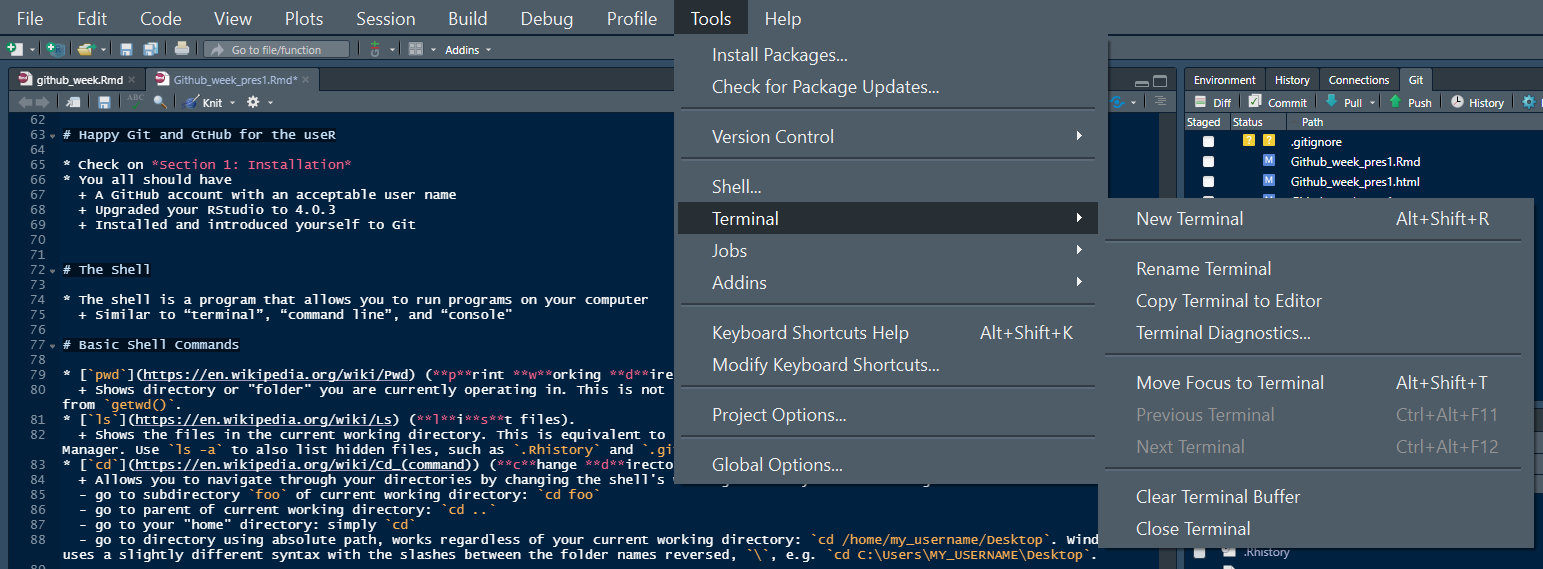
\includegraphics{pres_figs/terminal.png}

\end{frame}

\begin{frame}[fragile]{Basic Shell Commands}
\protect\hypertarget{basic-shell-commands}{}

\begin{itemize}
\tightlist
\item
  \href{https://en.wikipedia.org/wiki/Pwd}{\texttt{pwd}} (\textbf{p}rint
  \textbf{w}orking \textbf{d}irectory).

  \begin{itemize}
  \tightlist
  \item
    Shows directory or ``folder'' you are currently operating in.
  \end{itemize}
\item
  \href{https://en.wikipedia.org/wiki/Ls}{\texttt{ls}}
  (\textbf{l}i\textbf{s}t files).

  \begin{itemize}
  \tightlist
  \item
    Shows the files in the current working directory. This is equivalent
    to looking at the files in your Finder/Explorer/File Manager.
  \end{itemize}
\item
  \href{https://en.wikipedia.org/wiki/Cd_(command)}{\texttt{cd}}
  (\textbf{c}hange \textbf{d}irectory).

  \begin{itemize}
  \tightlist
  \item
    Allows you to navigate through your directories by changing the
    shell's working directory. You can navigate like so:
  \item
    go to subdirectory \texttt{foo} of current working directory:
    \texttt{cd\ foo}
  \item
    go to parent of current working directory: \texttt{cd\ ..}
  \item
    go to your ``home'' directory: simply \texttt{cd}
  \end{itemize}
\item
  Use arrow-up and arrow-down to repeat previous commands. Or search for
  previous commands with \texttt{CTRL} + \texttt{r}.
\end{itemize}

\end{frame}

\begin{frame}{Chapter 12: Connect RStudio to Git and GitHub}
\protect\hypertarget{chapter-12-connect-rstudio-to-git-and-github}{}

\begin{block}{Objectives:}

\begin{enumerate}
\tightlist
\item
  Make sure that you can all pull from and push to GitHub in RStudio on
  your local computer
\item
  Use RStudio to edit, commit, and push to your remote GitHub repo
\end{enumerate}

\end{block}

\begin{block}{Order of operation}

\begin{enumerate}
\tightlist
\item
  Connect to GitHub
\item
  Make a repository (or repo) on GitHub
\item
  Clone the repo to your local computer via RStudio
\item
  Make a local change, commit, and push
\item
  Confirm local change propagated to the GitHub remote
\item
  Clean up
\end{enumerate}

\end{block}

\end{frame}

\begin{frame}{Connect to GitHub}
\protect\hypertarget{connect-to-github}{}

\begin{itemize}
\tightlist
\item
  Start by going to \url{https://github.com} and logging in
\end{itemize}

\begin{figure}
\centering
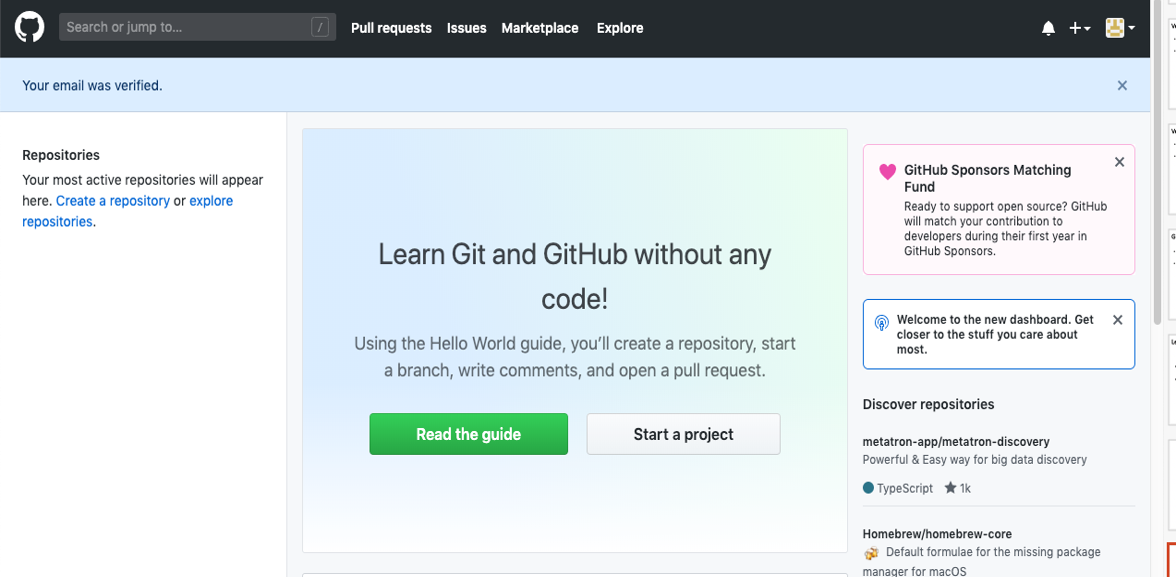
\includegraphics{pres_figs/homepage.png}
\caption{Homepage should look like this}
\end{figure}

\end{frame}

\begin{frame}{Make a repo on GitHub}
\protect\hypertarget{make-a-repo-on-github}{}

Click the plus, then the ``New repository'' button.

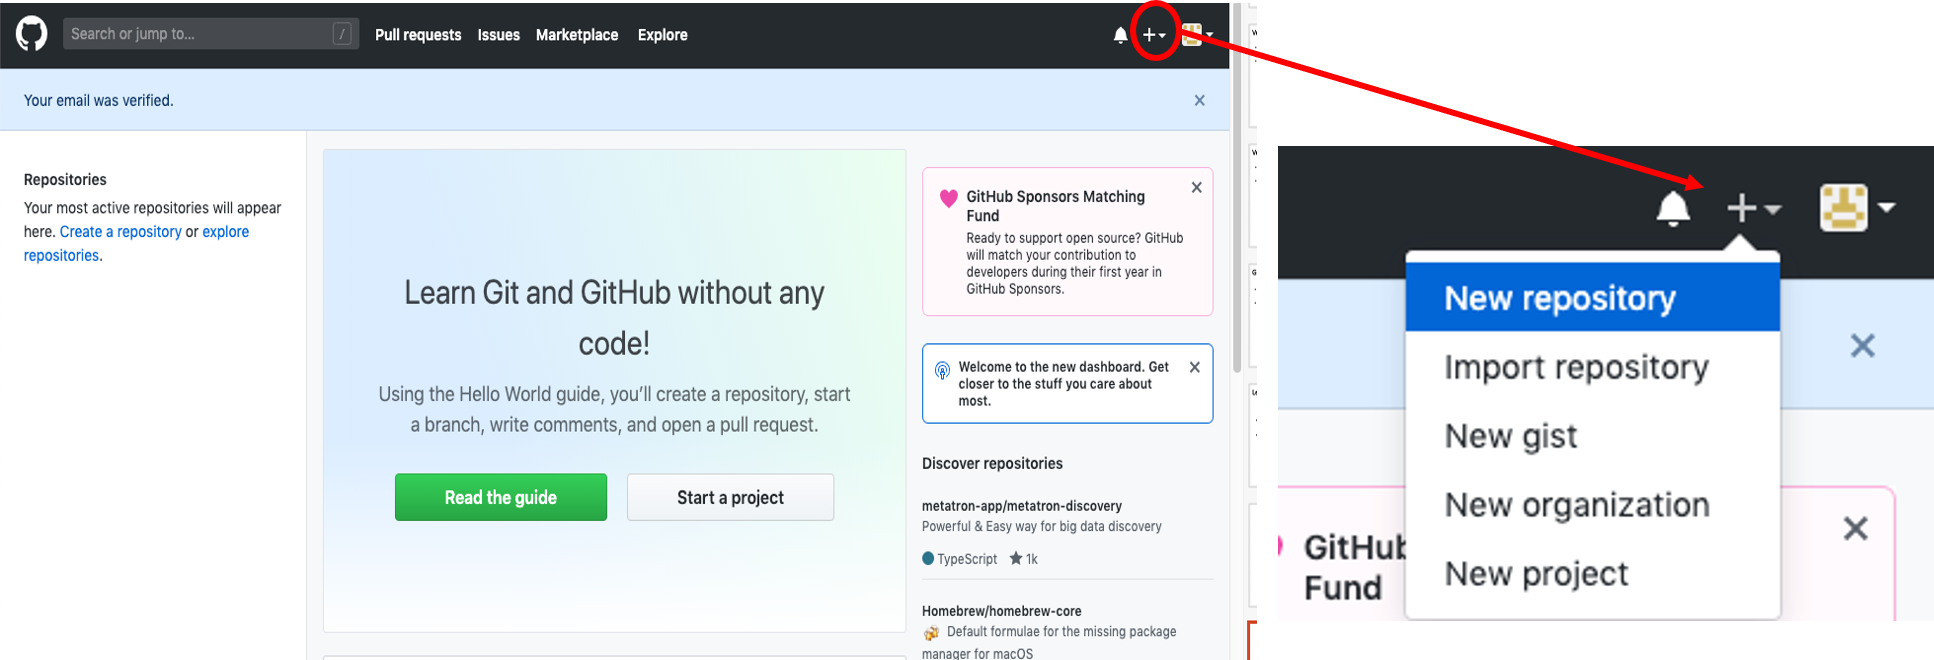
\includegraphics{pres_figs/new_repo.png}

\end{frame}

\begin{frame}[fragile]{Make a repo on GitHub}
\protect\hypertarget{make-a-repo-on-github-1}{}

\begin{columns}[T]
\begin{column}{0.48\textwidth}
\begin{itemize}
\tightlist
\item
  How to fill this in:

  \begin{itemize}
  \tightlist
  \item
    Repository name: \texttt{myrepo} (or whatever you wish, we'll delete
    this soon anyway).
  \item
    Description: ``testing my setup'' (or whatever, but some text is
    good for the README).
  \item
    Public.
  \item
    YES Initialize this repository with a README.
  \end{itemize}
\item
  For everything else, just accept the default.
\item
  Click big green button ``Create repository.''
\end{itemize}
\end{column}

\begin{column}{0.48\textwidth}
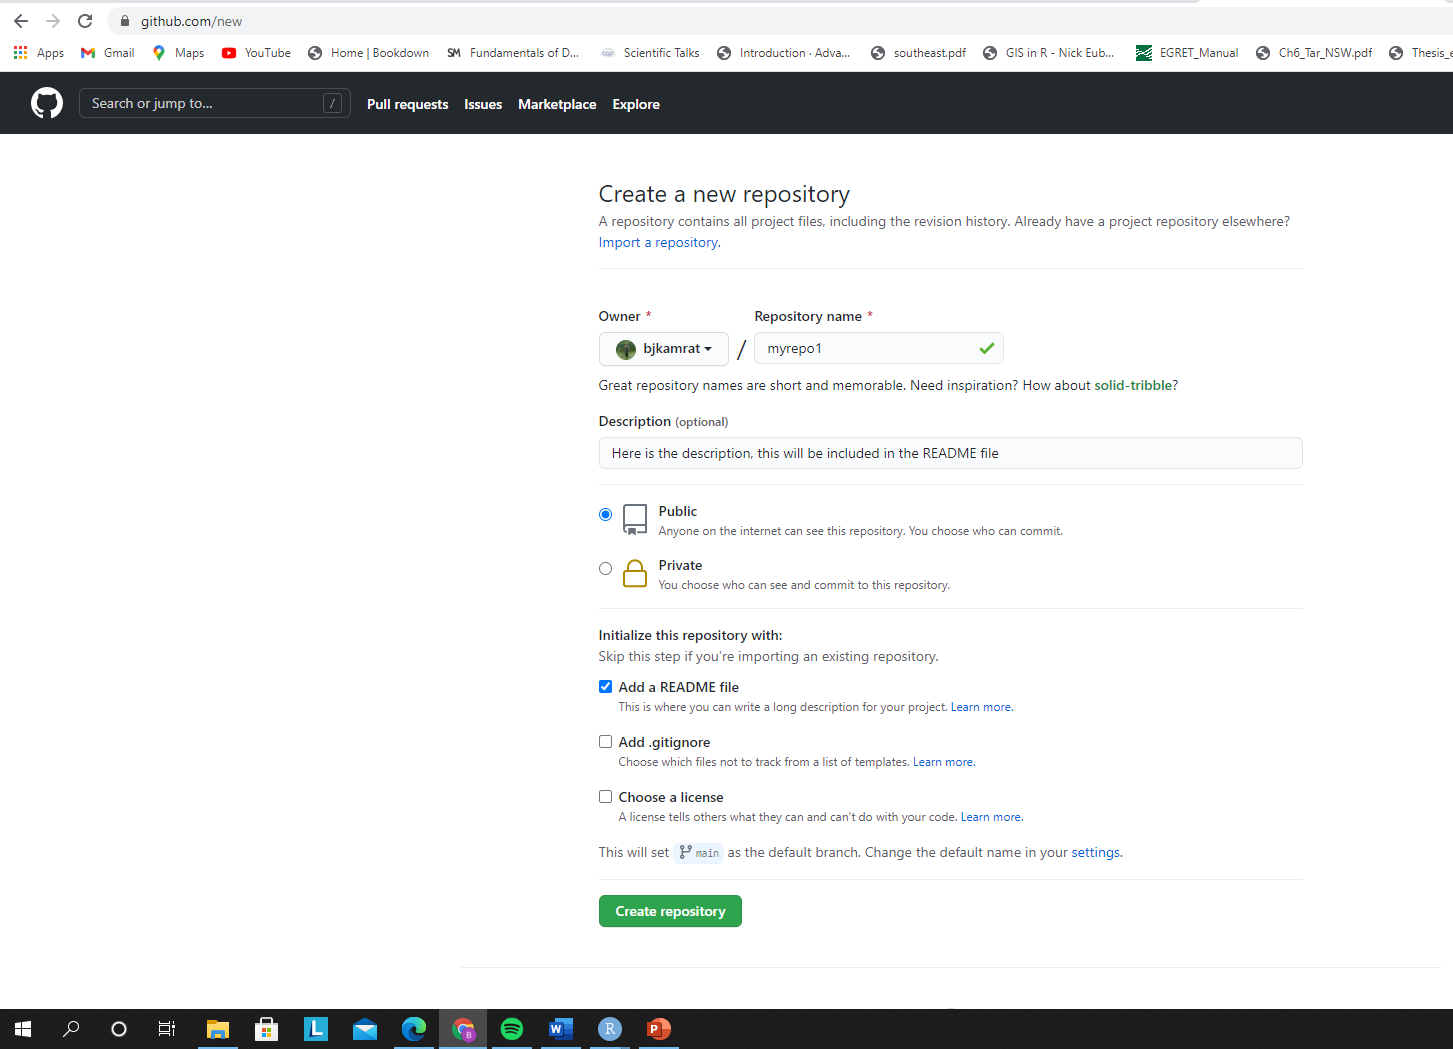
\includegraphics{pres_figs/new_repo_main.png}
\end{column}
\end{columns}

\end{frame}

\begin{frame}{Make a repo on GitHub}
\protect\hypertarget{make-a-repo-on-github-2}{}

\begin{figure}
\centering
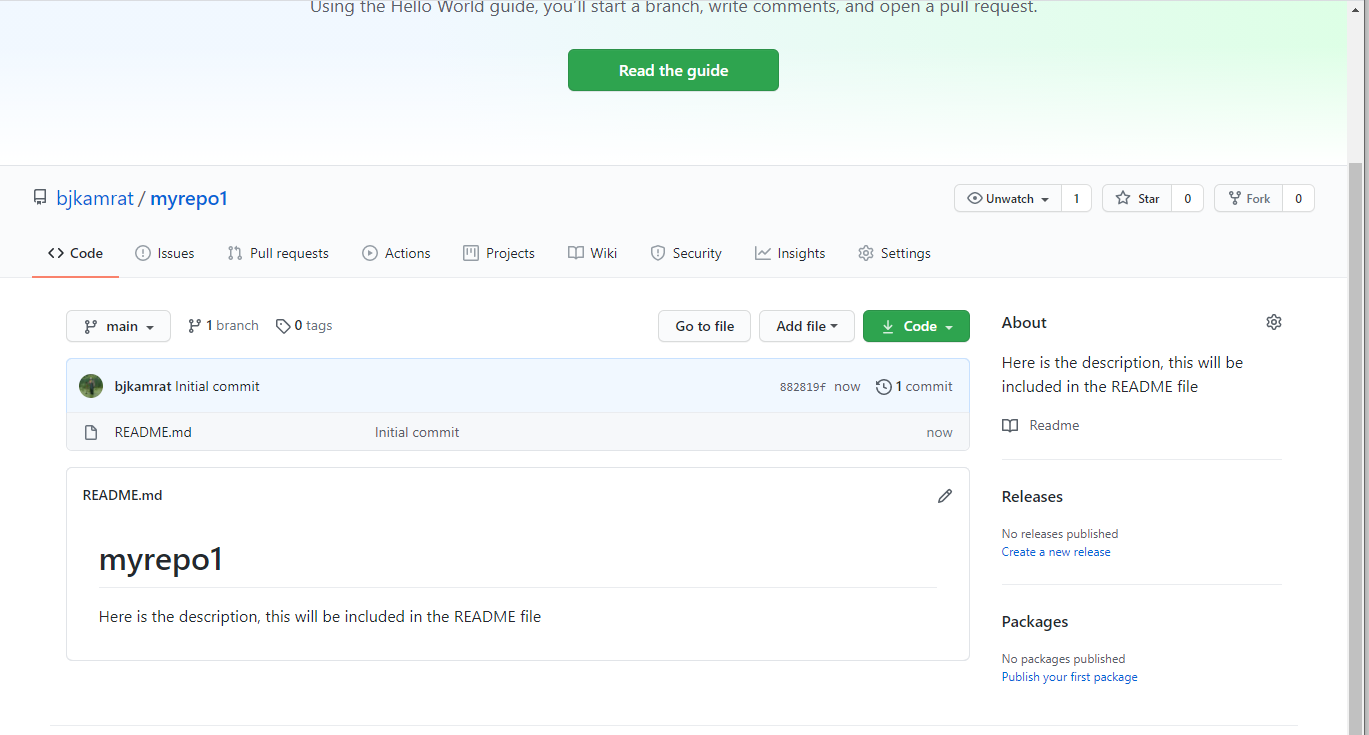
\includegraphics{pres_figs/new_repo_mainpage.png}
\caption{You should see this}
\end{figure}

\end{frame}

\begin{frame}{Clone the repo to your local computer}
\protect\hypertarget{clone-the-repo-to-your-local-computer}{}

Copy the HTTPS clone URL to your clipboard via the green ``Clone or
Download'' button.

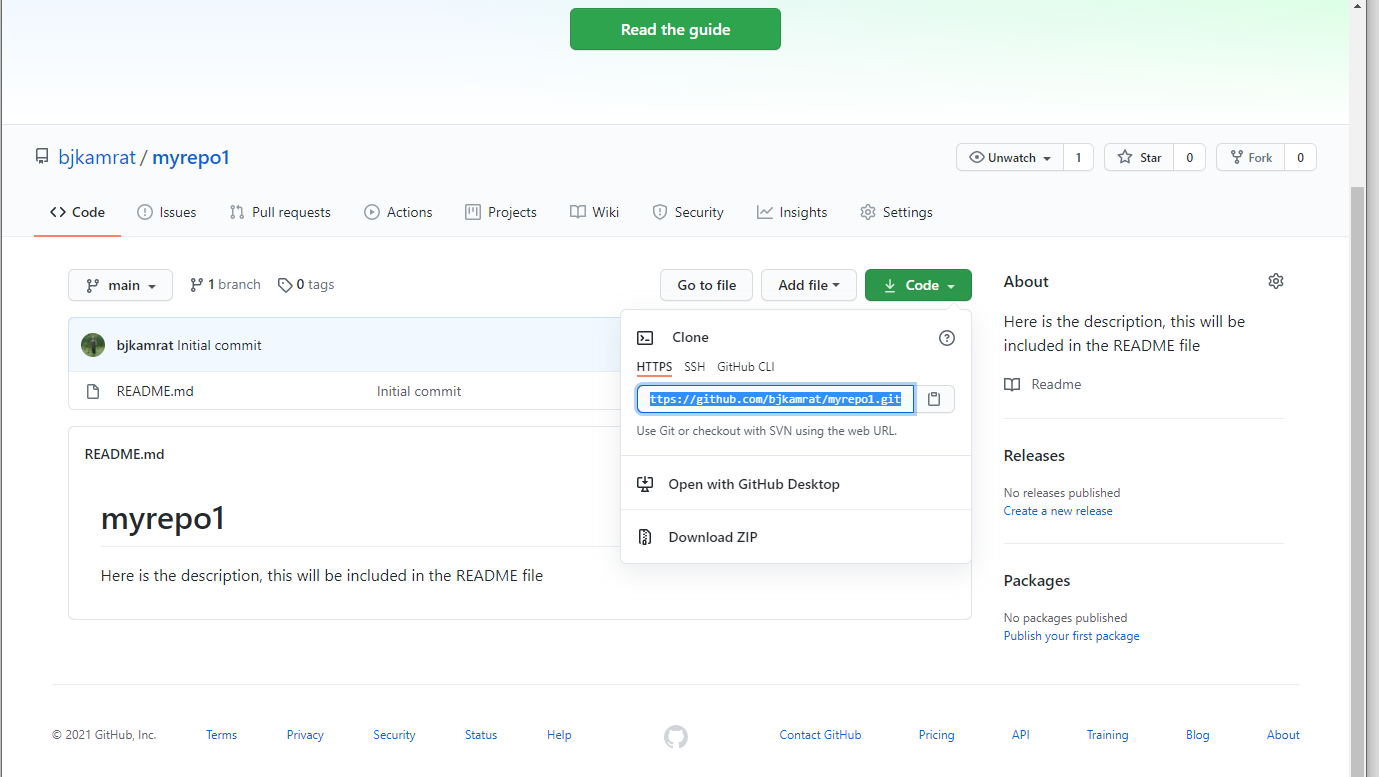
\includegraphics{pres_figs/clone.png}

\end{frame}

\begin{frame}[fragile]{Clone the new GitHub repo to your local computer
via RStudio}
\protect\hypertarget{clone-the-new-github-repo-to-your-local-computer-via-rstudio}{}

\begin{columns}[T]
\begin{column}{0.48\textwidth}
\begin{itemize}
\tightlist
\item
  Start a new Project in RStudio

  \begin{itemize}
  \tightlist
  \item
    \emph{File \textgreater{} New Project \textgreater{} Version Control
    \textgreater{} Git}.
  \item
    In the ``repository URL'' paste the URL of your new GitHub
    repository.

    \begin{itemize}
    \tightlist
    \item
      \texttt{https://github.com/bjkamrat/myrepo.git}
    \end{itemize}
  \end{itemize}
\item
  Be intentional about where you create this Project.
\item
  Check "Open in new session
\item
  Click ``Create Project'' to create a new directory, which will be:

  \begin{itemize}
  \tightlist
  \item
    a directory or ``folder'' on your computer
  \item
    a Git repository, linked to a remote GitHub repository
  \item
    an RStudio Project
  \end{itemize}
\end{itemize}
\end{column}

\begin{column}{0.48\textwidth}
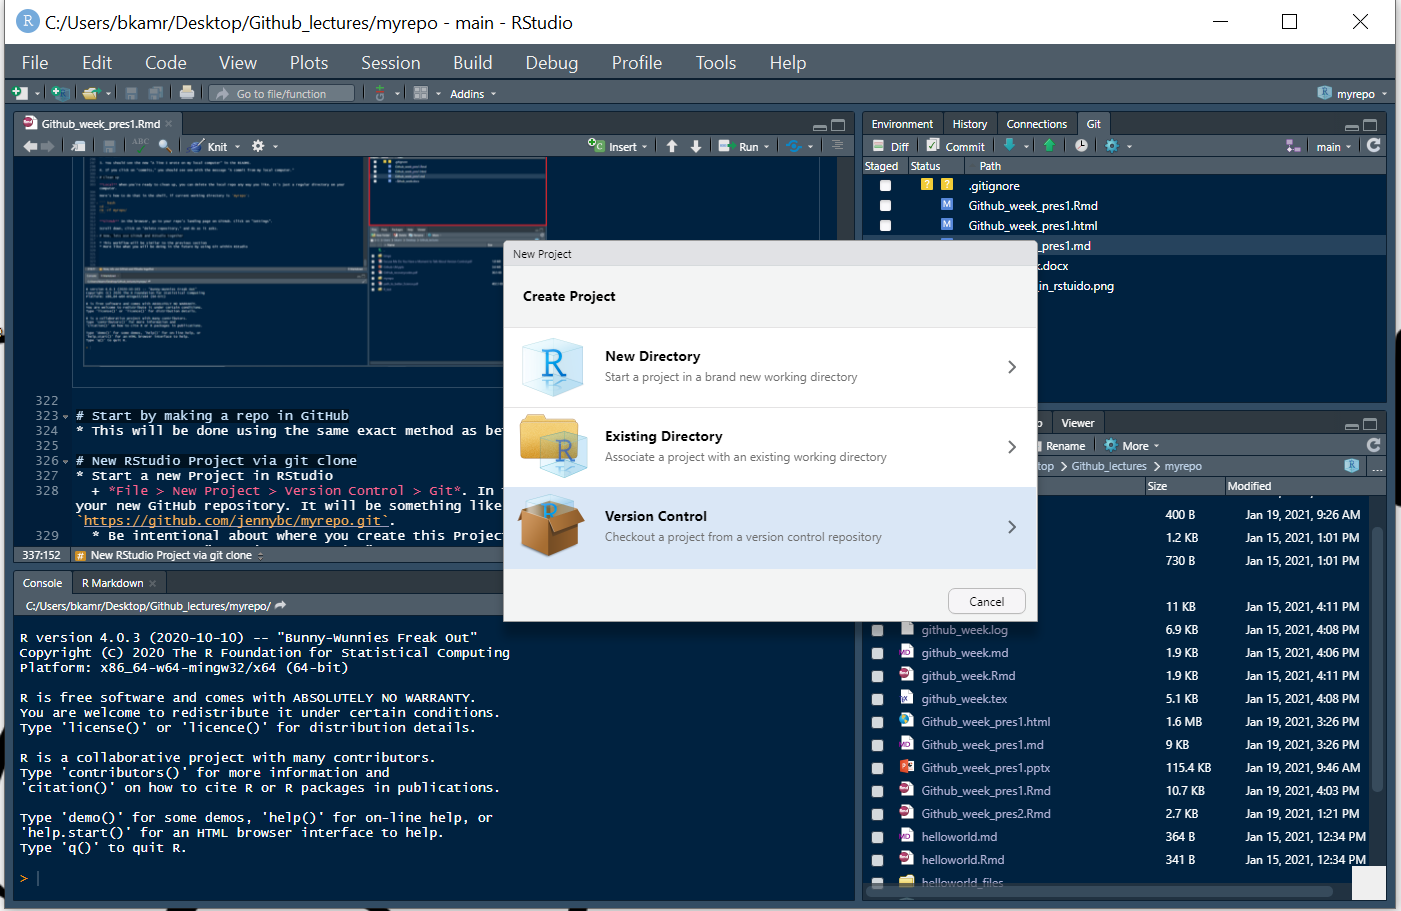
\includegraphics{pres_figs/new_project_rstudio.png}
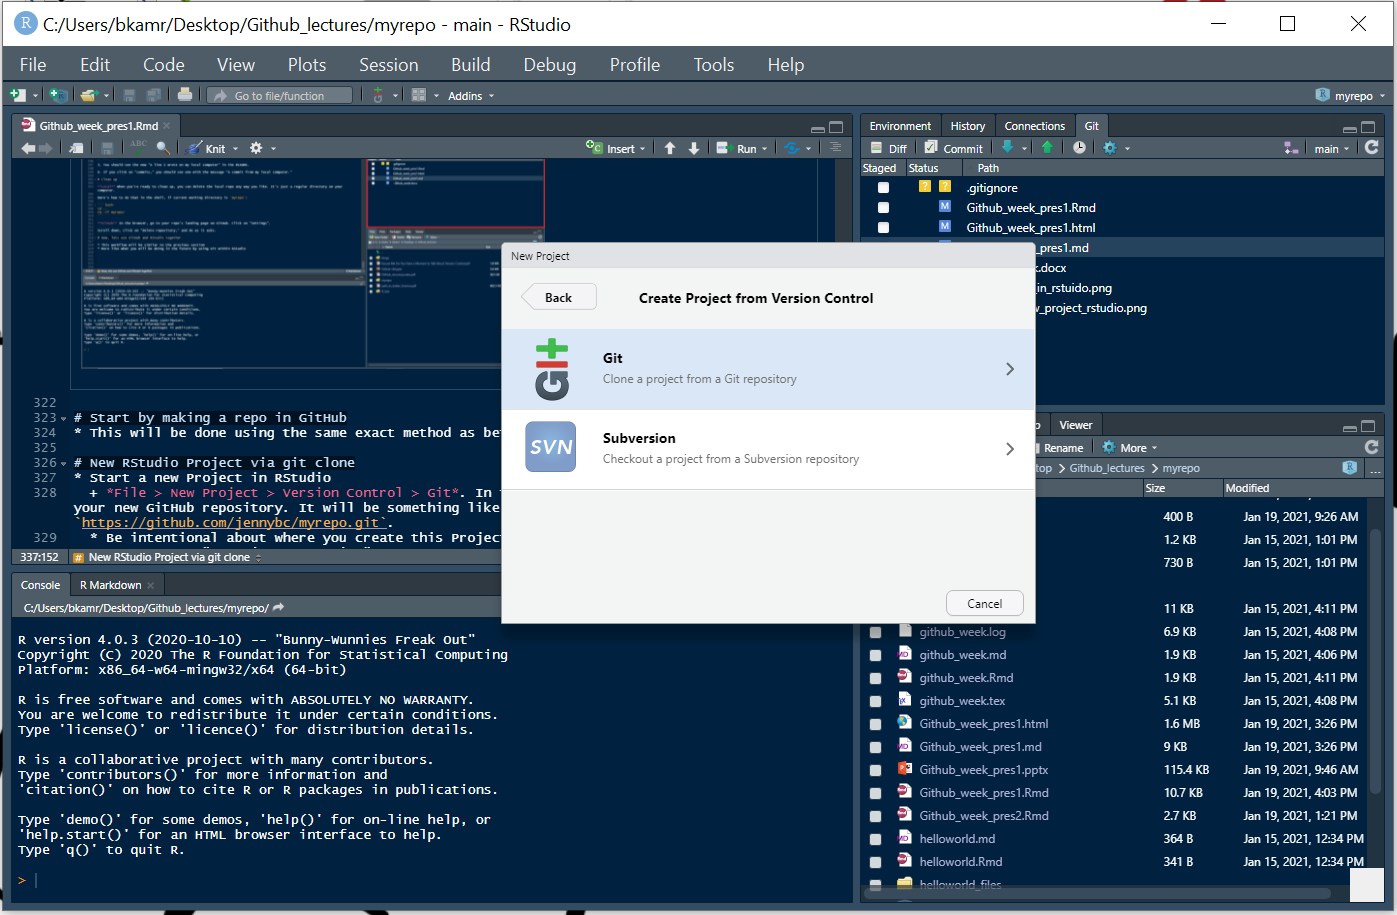
\includegraphics{pres_figs/new_project_rstudio_git.png}
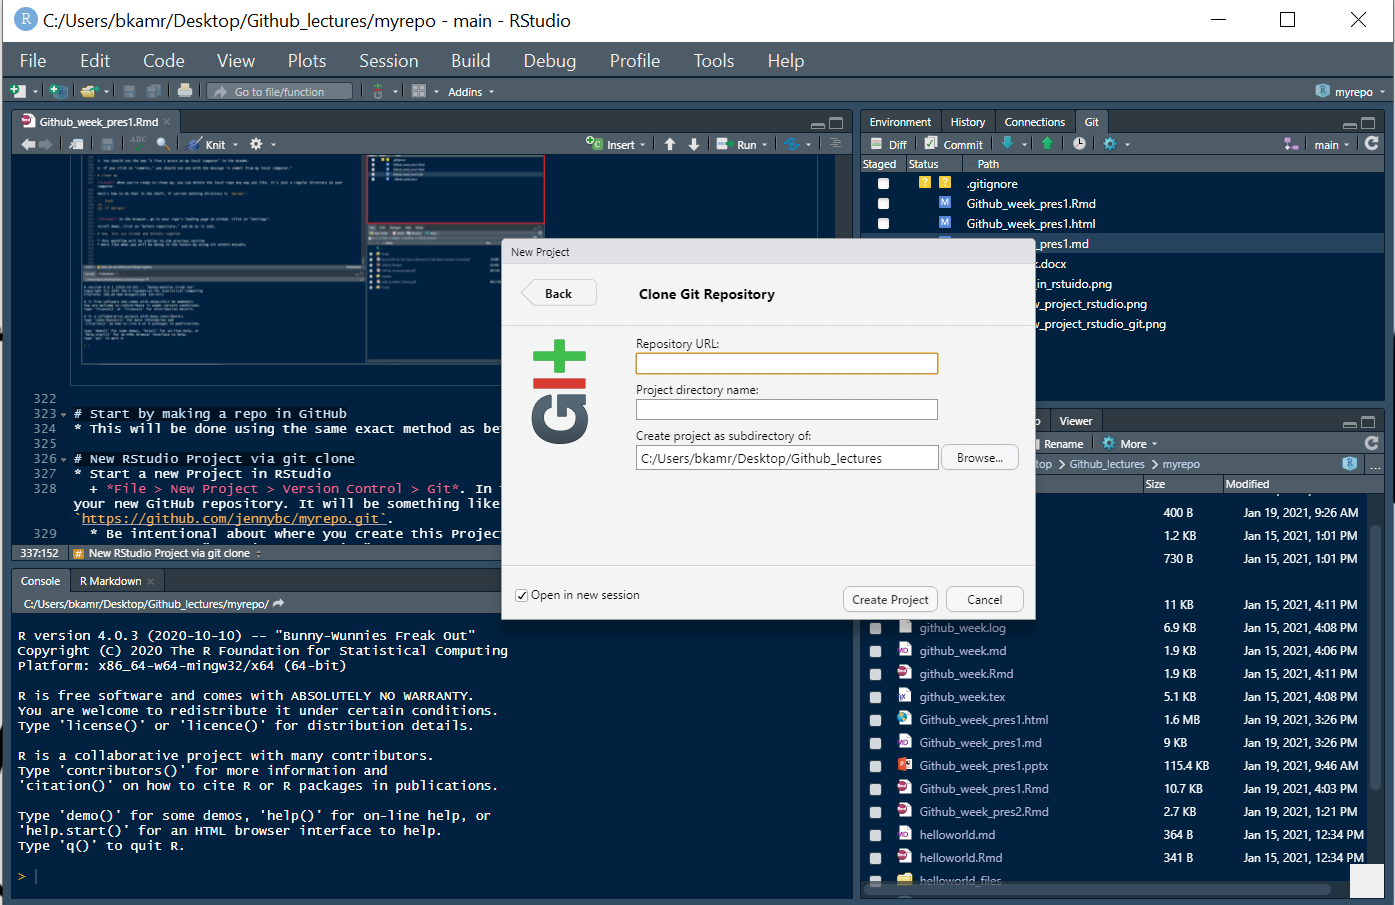
\includegraphics{pres_figs/new_project_rstudio_git_url.png}
\end{column}
\end{columns}

\begin{itemize}
\item
  \textbf{All of your R projects should have this set-up.}
\item
  The new local RStudio Project should represent the new test remote
  repo created on GitHub
\end{itemize}

\end{frame}

\begin{frame}[fragile]{Make a local change, commit, and push}
\protect\hypertarget{make-a-local-change-commit-and-push}{}

In your local RStudio Project modify the \texttt{README.md} file + Add
the line ``This is a line from RStudio'' + Save your change

\end{frame}

\begin{frame}[fragile]{Now, commit these changes to your local repo.
How?}
\protect\hypertarget{now-commit-these-changes-to-your-local-repo.-how}{}

In RStudio:

\begin{itemize}
\tightlist
\item
  Click the ``Git'' tab in upper right pane.
\item
  Click the white ``Staged'' box for \texttt{README.md}.
\item
  Click ``Commit''.
\item
  ``Comment'' on your ``commit''!

  \begin{itemize}
  \tightlist
  \item
    ``Commit message'', such as ``Commit from RStudio''.
  \end{itemize}
\item
  Click ``Commit''.
\end{itemize}

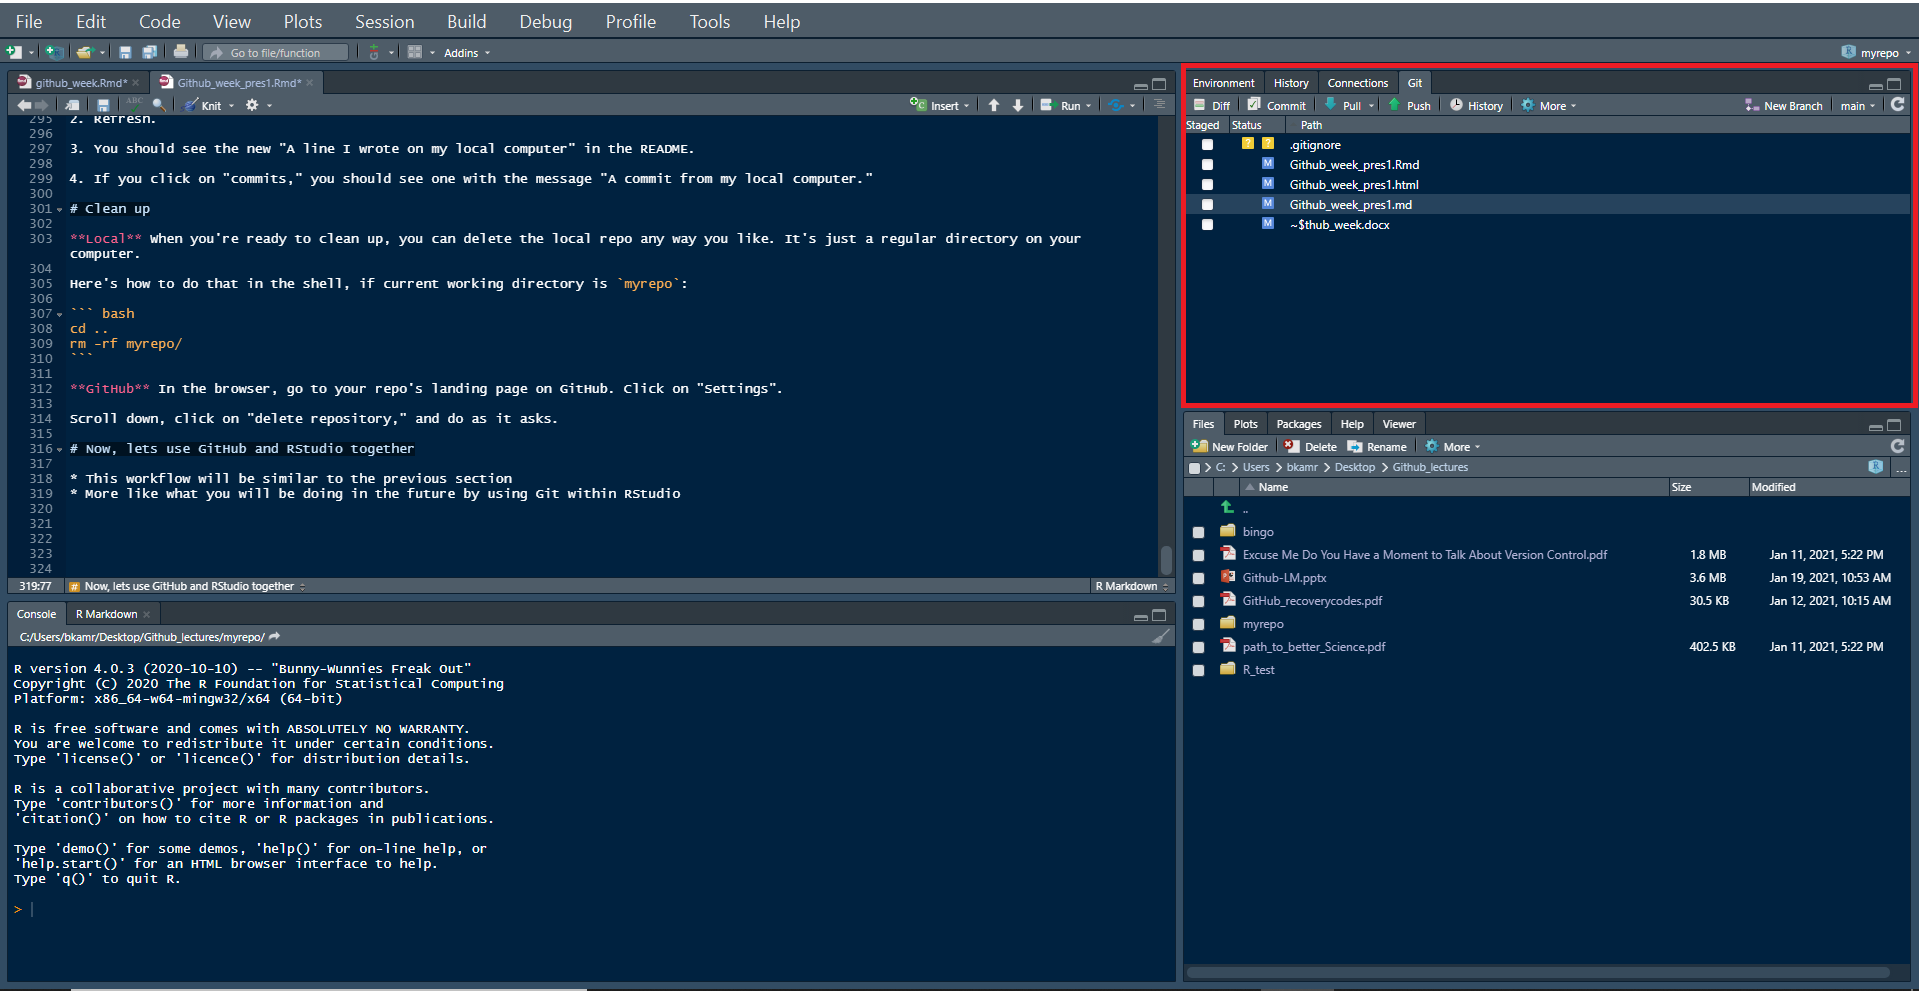
\includegraphics{pres_figs/git_in_rstuido.png}

\begin{block}{Pull then Push your local changes online to GitHub}

\begin{itemize}
\tightlist
\item
  First, Pull into RStudio the most updated verison of the GitHub Repo

  \begin{itemize}
  \tightlist
  \item
    You should see some message\ldots{}
  \end{itemize}
\end{itemize}

\begin{Shaded}
\begin{Highlighting}[]
\ExtensionTok{Already}\NormalTok{ up to date.}
\end{Highlighting}
\end{Shaded}

\begin{itemize}
\tightlist
\item
  Click the green ``Push'' button to send your local changes to GitHub.
  If you are challenged for username and password, provide them

  \begin{itemize}
  \tightlist
  \item
    You should see some message..
  \end{itemize}
\end{itemize}

\begin{Shaded}
\begin{Highlighting}[]
\NormalTok{[}\ExtensionTok{master}\NormalTok{ dc671f0] blah}
 \ExtensionTok{3}\NormalTok{ files changed, 22 insertions(+)}
 \ExtensionTok{create}\NormalTok{ mode 100644 .gitignore}
 \ExtensionTok{create}\NormalTok{ mode 100644 myrepo.Rproj}
\end{Highlighting}
\end{Shaded}

\end{block}

\end{frame}

\begin{frame}{Workflow}
\protect\hypertarget{workflow}{}

Do work somewhere. Commit it. Push it or pull it* depending on where you
did it, but get local and remote ``synced up''. Repeat.

* Note that in general (and especially in future when collaborating with
other developers) you will usually need to pull changes from the remote
(GitHub) before pushing the local changes you have made. For this
reason, it's a good idea to try and get into the habit of pulling before
you attempt to push.

\end{frame}

\begin{frame}{Confirm local change propgated to GitHub}
\protect\hypertarget{confirm-local-change-propgated-to-github}{}

\begin{enumerate}
\item
  Go back to the browser. I assume we're still viewing your new GitHub
  repo.
\item
  Refresh.
\item
  You should see the new ``This is a line from RStudio'' in the README.
\item
  If you click on ``commits,'' you should see one with the message
  ``Commit from Rstudio''
\end{enumerate}

\end{frame}

\begin{frame}{Clean up}
\protect\hypertarget{clean-up}{}

\textbf{Local} * When you're ready to clean up, you can delete the local
repo any way you like. It's just a regular directory on your computer.

\textbf{GitHub} * In the browser, go to your repo's landing page on
GitHub. Click on ``Settings''. * Scroll down, click on ``delete
repository,'' and do as it asks.

\end{frame}

\begin{frame}{}
\protect\hypertarget{section}{}

\includegraphics{https://media.giphy.com/media/ccRMvuh3PeuSGgOWVx/giphy.gif}

\end{frame}

\begin{frame}{Before moving on, lets discuss some of the Git
methodology/terminology}
\protect\hypertarget{before-moving-on-lets-discuss-some-of-the-git-methodologyterminology}{}

\begin{itemize}
\item
  Git allows you to take snapshots of all the files in a folder
\item
  This folder is your \emph{repository} or \emph{repo}
\item
  When you \emph{commit}, you take a snapshot, which you then
  \emph{push} to Github with a comment

  \begin{itemize}
  \tightlist
  \item
    Think of taking a picture (\emph{commit}) then posting
    (\emph{pushing}) the picture to instagram

    \begin{itemize}
    \tightlist
    \item
      and you wouldn't post a picture to instagram without a
      \emph{comment}
    \end{itemize}
  \end{itemize}
\end{itemize}

\end{frame}

\begin{frame}{Git methodology/terminology}
\protect\hypertarget{git-methodologyterminology}{}

\begin{itemize}
\tightlist
\item
  When you \emph{commit} a file or files, additional information is
  saved along with the changes to the file

  \begin{itemize}
  \tightlist
  \item
    Who
  \item
    When
  \item
    What was changed
  \item
    A comment on the change
  \end{itemize}
\end{itemize}

\end{frame}

\begin{frame}{Git methodology/terminology}
\protect\hypertarget{git-methodologyterminology-1}{}

These snapshots act as version control

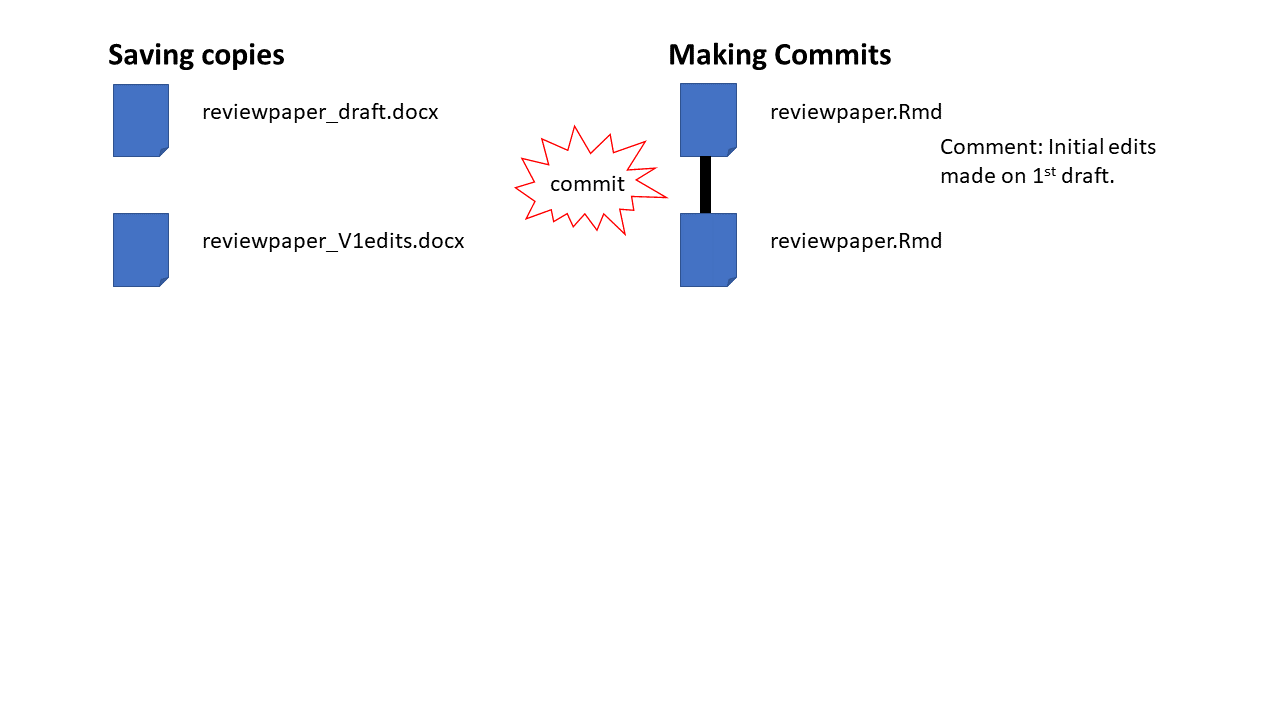
\includegraphics{pres_figs/copies_commits1.png}

\end{frame}

\begin{frame}{Git methodology/terminology}
\protect\hypertarget{git-methodologyterminology-2}{}

These snapshots act as version control

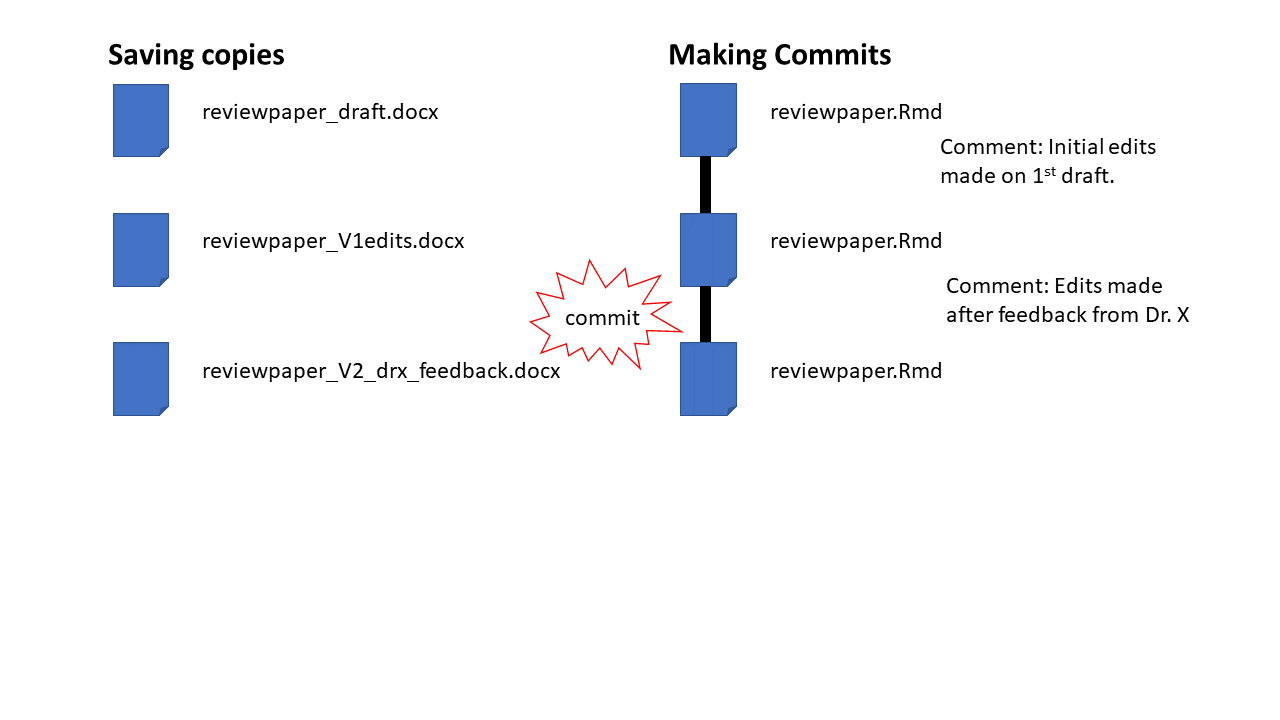
\includegraphics{pres_figs/copies_commits2.png}

\end{frame}

\begin{frame}{Git methodology/terminology}
\protect\hypertarget{git-methodologyterminology-3}{}

These snapshots act as version control

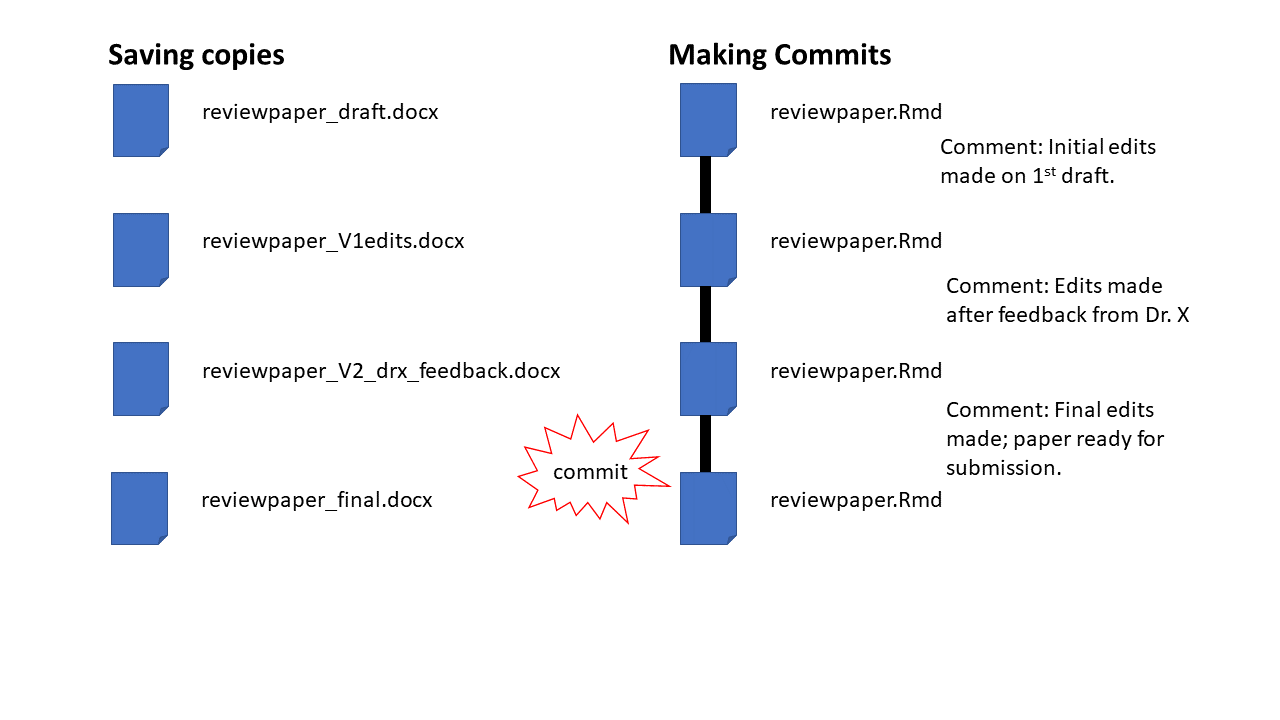
\includegraphics{pres_figs/copies_commits3.png}

\end{frame}

\begin{frame}{Git methodology/terminology}
\protect\hypertarget{git-methodologyterminology-4}{}

\begin{itemize}
\tightlist
\item
  Git, or in our case GitHub, stores the history of your project

  \begin{itemize}
  \tightlist
  \item
    This lets you time travel to different versions of your project
  \item
    you can \emph{check out} these older versions of the project
  \end{itemize}
\end{itemize}

\end{frame}

\begin{frame}{Git methodology/terminology}
\protect\hypertarget{git-methodologyterminology-5}{}

\begin{itemize}
\tightlist
\item
  What if you want to experiment with making some changes to files in
  your project?

  \begin{itemize}
  \tightlist
  \item
    you can do this by creating a \emph{branch}
  \end{itemize}
\item
  A \emph{branch} is a moveable label attached to a commit
\end{itemize}

\end{frame}

\begin{frame}{Git methodology/terminology}
\protect\hypertarget{git-methodologyterminology-6}{}

\begin{itemize}
\tightlist
\item
  The default \emph{branch} name in GitHub is \emph{master}

  \begin{itemize}
  \tightlist
  \item
    To experiment with making some changes created a new \emph{branch}
  \item
    If you are happy with the changes you can \emph{merge} them back
    into the \emph{master}
  \end{itemize}
\item
  In collaborative projects

  \begin{itemize}
  \tightlist
  \item
    most changes should be done in a new \emph{branch}
  \item
    the \emph{master} \emph{branch} is often the verison of the code
    that is published on a site
  \end{itemize}
\end{itemize}

\end{frame}

\begin{frame}{Git methodology/terminology}
\protect\hypertarget{git-methodologyterminology-7}{}

\begin{itemize}
\tightlist
\item
  As you know, it is always good to back up your work

  \begin{itemize}
  \tightlist
  \item
    Typically, not on your local computer
  \end{itemize}
\item
  This outside storage location is called a \emph{remote}

  \begin{itemize}
  \tightlist
  \item
    GitHub is one very popular \emph{remote}
  \end{itemize}
\end{itemize}

\end{frame}

\begin{frame}{Git methodology/terminology}
\protect\hypertarget{git-methodologyterminology-8}{}

\begin{itemize}
\item
  To get work from a \emph{remote} for the first time you must
  \emph{clone} it to your local computer \_ We just did this!!
\item
  If you make a change at the local level,

  \begin{enumerate}
  \tightlist
  \item
    You can \emph{commit} the change
  \item
    Then \emph{push} it back to the remote
  \item
    For someone else to have the most updated repo, they now need to
    \emph{pull} your changes to their local computer
  \end{enumerate}
\end{itemize}

\end{frame}

\begin{frame}{Summary}
\protect\hypertarget{summary}{}

\emph{repo} - your project folder

\emph{commit} - snapshot of repo

\emph{checkout} - time travel to specific commit

\emph{branch} - a moveable label that point to a commit

\emph{merge} - combining two branches

\emph{remote} - a computer/server with the repository on it

\emph{clone} - the first time you get the repo from the remote

\emph{push} - send commits (with comments) to a remote

\emph{pull} - get updated repo from a remote

\begin{itemize}
\tightlist
\item
  Haven't yet discussed
\item
  \emph{fork} or \emph{pull request} or \emph{upstream}
\end{itemize}

\end{frame}

\begin{frame}{}
\protect\hypertarget{section-1}{}

\includegraphics{https://media.giphy.com/media/SwBtg47JjsOU9QZuW0/giphy.gif}

\end{frame}

\begin{frame}{Now, lets use GitHub and RStudio together (Chapter 15)}
\protect\hypertarget{now-lets-use-github-and-rstudio-together-chapter-15}{}

\begin{itemize}
\tightlist
\item
  This workflow will be similar to the previous section
\item
  More like what you will be doing in the future by using Git within
  RStudio
\end{itemize}

\end{frame}

\begin{frame}[fragile]{Start by making a repo in GitHub}
\protect\hypertarget{start-by-making-a-repo-in-github}{}

\begin{itemize}
\tightlist
\item
  This will be done using the same exact method as before
\item
  Remember

  \begin{itemize}
  \tightlist
  \item
    Repository name: \texttt{myrepo} (or whatever you wish, we'll delete
    this soon anyway).
  \item
    Description: ``testing my setup'' (or whatever, but some text is
    good for the README).
  \item
    Public.
  \item
    YES Initialize this repository with a README.
  \end{itemize}
\item
  For everything else, just accept the default.
\item
  Click big green button ``Create repository.''
\end{itemize}

\end{frame}

\begin{frame}{From here}
\protect\hypertarget{from-here}{}

\begin{itemize}
\tightlist
\item
  With the rest of the class period, I would like you to work on CH 15
  and go through CH 16 and 17.
\end{itemize}

For Thursday (2/4/21), you need to

\begin{itemize}
\tightlist
\item
  Complete Chapter 15
\item
  Finish reading Byran article (Excuse Me\ldots{})
\end{itemize}

\end{frame}

\end{document}
